\documentclass[11pt]{article}

\usepackage[margin=1in]{geometry}
\usepackage{graphicx}
\usepackage{hyperref}
\usepackage{setspace}
\usepackage{array}
\usepackage{float}
\usepackage{caption}

\setstretch{1.15}
\hypersetup{
    colorlinks=true,
    linkcolor=black,
    urlcolor=blue
}

\title{\vspace{-1.5cm}\textbf{CS 639 Final Project}\\
\large Attention-Based Context Compaction for Agentic Coding}
\author{Team Members: Arjun Sahlot, Anuj Sheth}
\date{\today}

\begin{document}

\maketitle
\vspace{-0.5cm}

\section*{Overarching Idea and Motivation}

Long-running coding agents accumulate a large amount of conversational state:
system instructions, user requests, chain-of-thought-like scratch work, tool
schemas, file reads, shell outputs, failed plans, partial edits, test failures,
and final answers. In traditional programming, garbage collection removes
objects that are no longer reachable or useful to future execution. Our project
started from the question of whether an analogous idea could be applied to the
context window of an agent: can we identify context that is no longer useful and
remove it while preserving the information the model still needs to solve the
task?

This motivation matters even as models support larger context windows. Larger
windows are not free: they increase latency, memory pressure, and cost, and they
can make it harder for the model to attend to the small subset of tokens that are
actually relevant to the next action. Coding agents are especially sensitive to
this because many steps are highly local. The model often needs a specific test
failure, a function signature, or a recent tool result, not every intermediate
mistake that occurred earlier in the run. Our goal was therefore to build a
research harness where we could inspect, score, visualize, and eventually prune
agent context during realistic coding tasks.

\section*{Basic Hypothesis}

Our original hypothesis was that keeping only the most important parts of the
previous prompts and responses could act like a low-rank or sparse approximation
of the conversation. The compressed context would not reproduce the entire
history, but it would preserve the features most useful for future prediction
and action. If this worked, an agent could run for more steps with a smaller
effective context window, lower memory pressure, and less distraction from stale
or irrelevant text.

During the project we refined this hypothesis into a more testable version:
attention received from future generated tokens can be used as an approximate
importance signal for previous prompt tokens. Tokens that repeatedly receive
attention during decoding are treated as more likely to matter for the model's
next decisions. Tokens with low normalized importance are candidates for
removal, while recent messages are preserved verbatim to avoid losing the latest
tool interaction.

\section*{What We Built}

We built a modular agentic coding harness rather than only a standalone
importance-analysis script. The final repository contains four major pieces:

\begin{itemize}
    \item \textbf{Local inference engine:} A HuggingFace and PyTorch based
    inference layer in \texttt{inference/}. It loads local causal language
    models, supports CUDA execution and optional quantization, streams tokens,
    reuses the KV cache during generation, and exposes generation statistics.

    \item \textbf{Agent loop and tools:} A minimal coding-agent loop in
    \texttt{harness/}. The agent can read files, write files, search with
    ripgrep, and run shell commands. Tool calls are represented explicitly in
    the conversation so the full state can be inspected and modified.

    \item \textbf{Web inspection interface:} A FastAPI server and React/Vite
    frontend in \texttt{server/} and \texttt{web/}. The UI streams model output,
    displays tool calls and results, supports manual context insertion, and
    visualizes token-level attention importance.

    \item \textbf{Benchmark runner:} A headless benchmark system in
    \texttt{scripts/run\_task\_benchmark.py} and \texttt{tasks/}. The tasks are
    self-contained Python repair problems with failing tests, maintainer context,
    and estimated context sizes around ten to fourteen thousand tokens.
\end{itemize}

This platform was a substantial part of the project. It gave us the control we
needed over the prompt, model outputs, tool history, attention capture, and
context-reduction policy. Existing production coding agents usually hide these
details, which makes them hard to use for controlled context-management
experiments.

\section*{Methodology}

Our methodology followed the structure of the original proposal, but we focused
our implementation effort on the parts needed to make the experiment observable.

\subsection*{1. Build a Custom Agent Harness}

We first implemented a simple but complete coding agent. The agent receives a
task prompt, renders the full chat history and tool schemas into a model prompt,
streams model output, parses XML-wrapped JSON tool calls, executes approved
tools, records tool results, and repeats until the model stops requesting tools
or the maximum round count is reached. This let us control the exact context
passed to the model at every generation step.

\subsection*{2. Capture Attention-Derived Token Importance}

The inference engine can optionally collect attention during decoding. To avoid
the largest memory blowup, we do not capture full prompt prefill attention.
Instead, every \texttt{N} generated tokens, the engine requests attention tensors
for the newest decode step. For each observed decode query, we accumulate how
much attention earlier key/value positions receive. We also weight deeper layers
slightly more and give more weight to lower-entropy heads, since focused
attention is a stronger signal than diffuse attention.

The raw scores are normalized by the 95th percentile of positive scores and
stored as a payload containing tokenizer pieces, token ids, raw scores,
normalized scores, and whether each token came from the prompt or generated
response. This gives us a concrete, inspectable measure of what prior text the
model appeared to use while producing later tokens.

\subsection*{3. Visualize Importance}

We added an attention heatmap UI so the scores were not just numbers in a log.
The frontend displays actual tokenizer pieces with color intensity based on
normalized importance. This made it much easier to debug whether the signal was
reasonable and to see which pieces of a response or prompt were being treated as
important.

\begin{figure}[H]
    \centering
    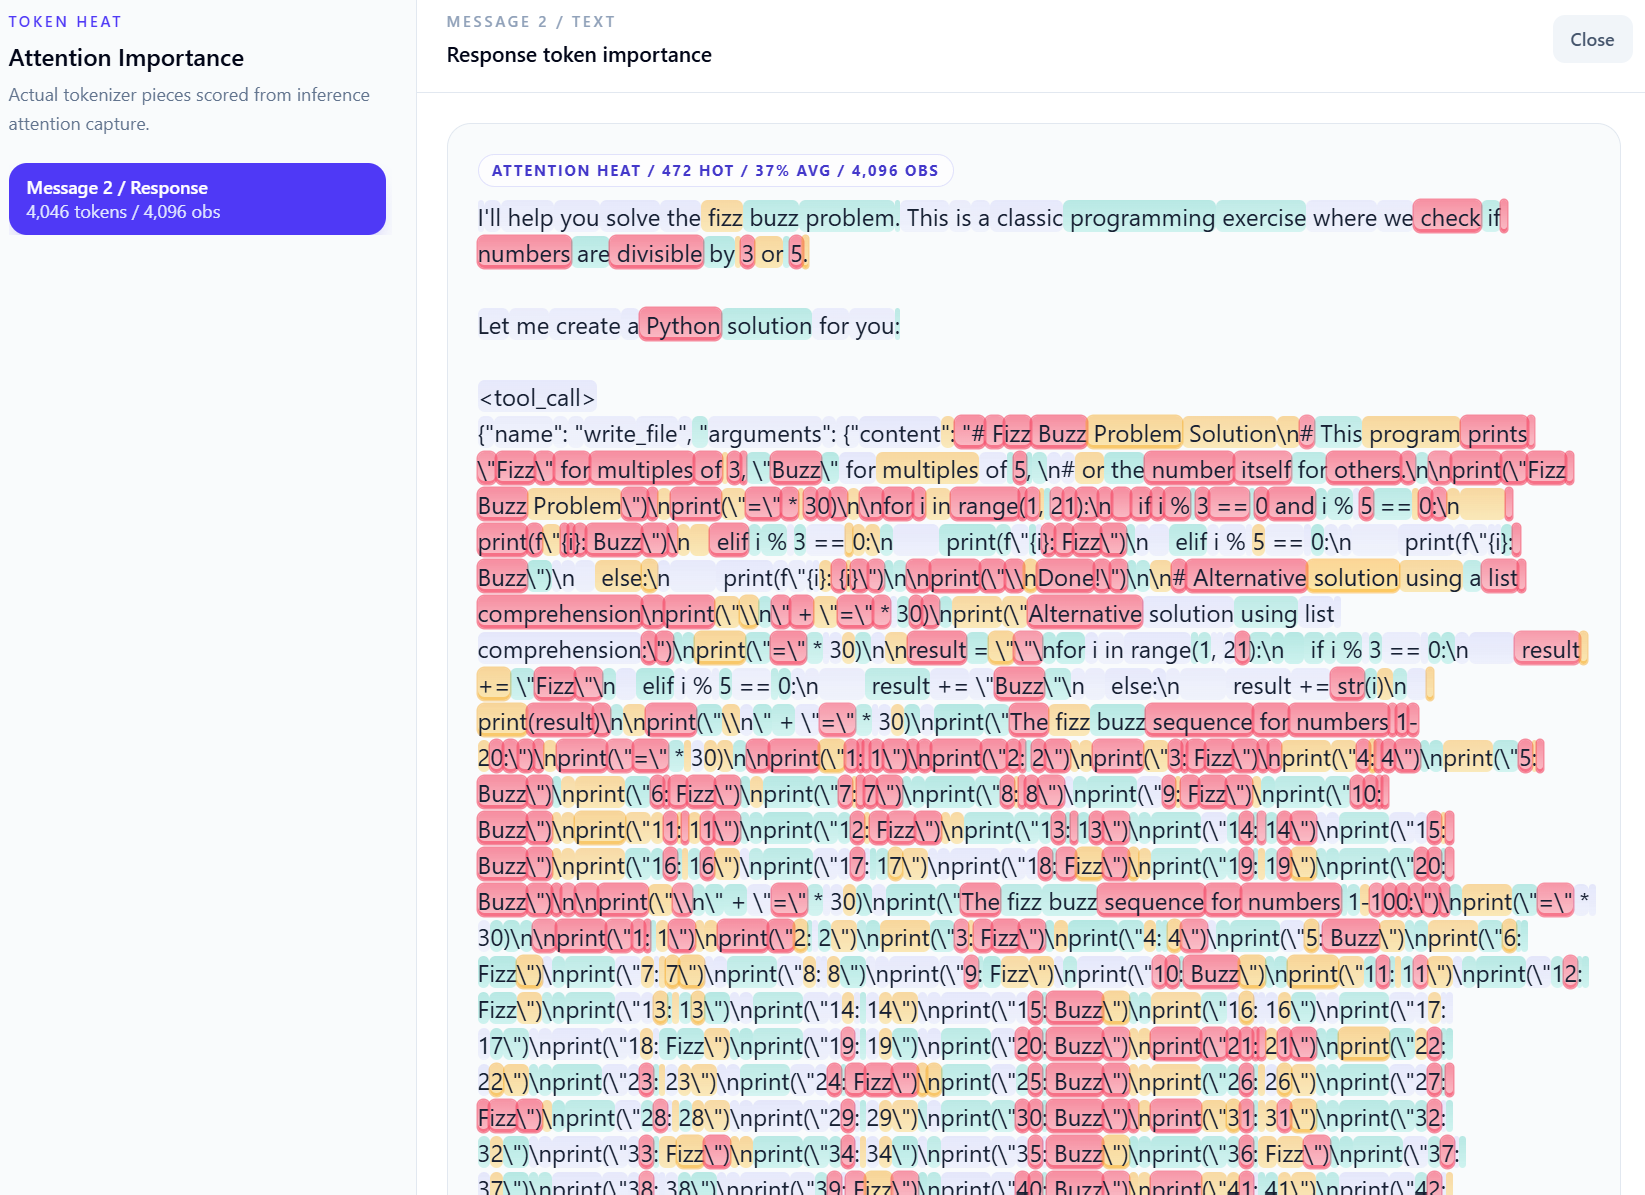
\includegraphics[width=\textwidth]{figures/importances.png}
    \caption{Token-level attention importance visualization from the web
    interface. The highlighted tokenizer pieces show which generated tokens
    received higher future-attention scores during a FizzBuzz-style coding
    response.}
    \label{fig:importance-heat}
\end{figure}

\subsection*{4. Implement Importance-Based Context Reduction}

We implemented an experimental reducer for the benchmark runner. After a model
round, the reducer can take the latest importance payload and select eligible
prompt tokens. It filters out empty and special tokens, ranks by normalized
importance, trims a configurable number of low-importance tokens, and reconstructs
a fragmentary ``importance-reduced context'' message in original token order.
The reducer also keeps the system prompt and the most recent non-system messages
verbatim. This design intentionally prioritizes not breaking the current tool
loop while still reducing older history.

\begin{figure}[H]
    \centering
    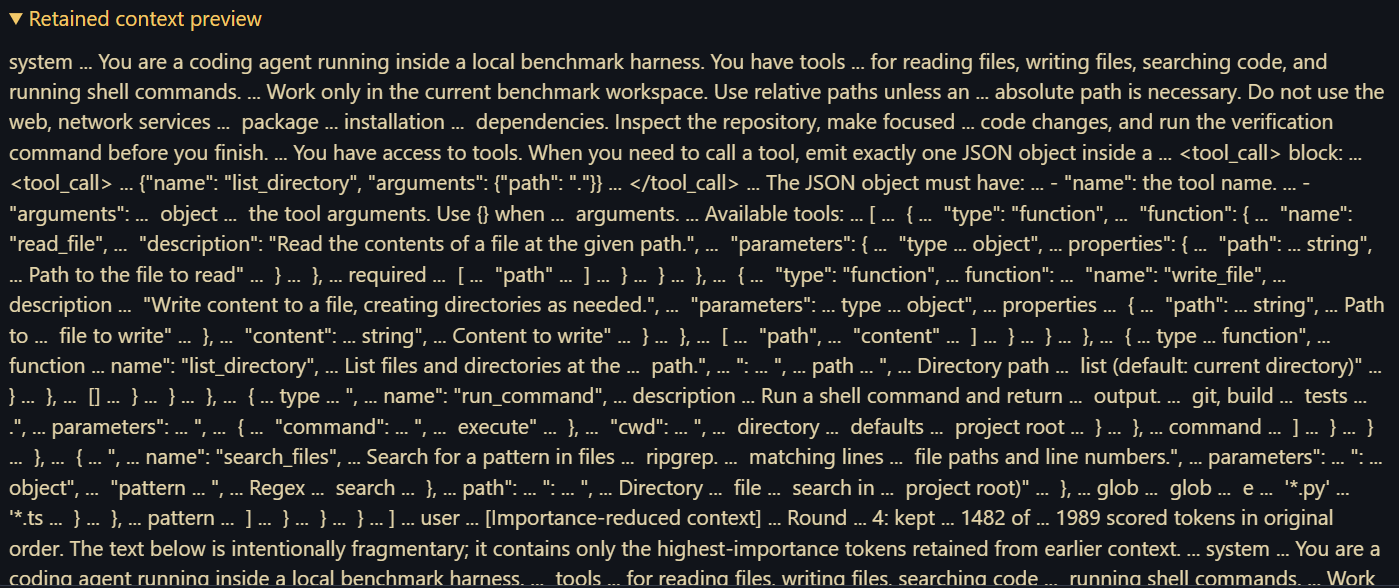
\includegraphics[width=\textwidth]{figures/retained.png}
    \caption{Retained context preview from an importance-reduced run. The
    preview shows that the reducer keeps high-scoring fragments from older
    context and explicitly marks the result as fragmentary rather than pretending
    to preserve a fluent summary.}
    \label{fig:retained-context}
\end{figure}

\subsection*{5. Benchmark on Long-Horizon Coding Tasks}

We created a suite of local software-engineering tasks. Each task contains a
small Python repository, failing implementations, tests, README files, fixtures,
and maintainer-context documents. The benchmark copies each task into a fresh
run directory, lets the agent edit the code, and then scores the result by
running \texttt{python -m unittest discover -s tests -v}. This gives a
repeatable setting for comparing base runs against context-reduced runs.

\section*{Progress and Preliminary Results}

By the end of the project, we reached a working end-to-end system:

\begin{itemize}
    \item local model loading and token streaming work through the custom engine;
    \item the agent can call file, search, and shell tools;
    \item attention-derived token importance is captured during generation;
    \item the UI visualizes token heatmaps for generated text;
    \item the benchmark runner can execute multi-task coding evaluations;
    \item the benchmark runner includes an importance-based context-reduction
    mode with JSON audit output and realtime monitor cards.
\end{itemize}

We also obtained a baseline benchmark run across twelve generated coding tasks.
The run did not solve any task completely, but it did make partial progress on
several tasks and passed 14 of 85 unit tests overall.

\begin{center}
\begin{tabular}{|>{\raggedright\arraybackslash}p{0.42\textwidth}|c|c|}
\hline
\textbf{Task} & \textbf{Score} & \textbf{Status} \\
\hline
csv\_schema\_migrator & 0/7 & Fail \\
event\_store\_snapshots & 6/7 & Fail \\
feature\_flags & 0/8 & Error \\
inventory\_forecast & 3/7 & Fail \\
ledger\_proration & 0/7 & Error \\
license\_audit & 0/8 & Fail \\
line\_diff\_reporter & 4/7 & Fail \\
log\_window\_rollups & 0/6 & Fail \\
markdown\_outline & 0/6 & Fail \\
route\_planner & 0/6 & Fail \\
semver\_resolver & 1/8 & Fail \\
template\_engine & 0/8 & Error \\
\hline
\textbf{Overall} & \textbf{14/85} & \textbf{Preliminary} \\
\hline
\end{tabular}
\end{center}

The result is best interpreted as evidence that the infrastructure works, not as
evidence that the final compaction method is already superior. The harness was
able to run real coding tasks, make edits, call tools, execute tests, and collect
the data needed for context-management experiments. The partial scores show that
the agent was interacting with the repositories meaningfully, but the local model
and compute budget were not sufficient to produce strong end-task success.

\section*{Compute and Time Limitations}

The biggest limitation was compute. Attention capture is expensive because it
requires eager attention tensors rather than the most optimized attention path.
Full prefill attention over long prompts is especially memory-intensive, so we
had to skip it and sample attention during decoding instead. Even with sampling
every several tokens, each benchmark run required loading a local model, running
many forward passes, preserving KV cache state, executing tools, and running test
suites across multiple repositories.

Time was the second major limitation. Building the harness, UI, benchmark
runner, task generator, scoring pipeline, and importance reducer took most of
the project window. As a result, we did not finish the full experimental matrix
we originally wanted: multiple models, multiple context sizes, sliding-window
baselines, summary-memory baselines, retrieval baselines, and repeated trials for
statistical confidence. We also did not fully tune the reducer. The current
reconstruction method is intentionally simple: it preserves high-importance
token fragments in order. This is useful for auditing and first experiments, but
it can produce unnatural context that may be harder for a model to use than a
structured summary.

\section*{Discussion}

The most promising outcome is that attention-based importance is now observable
inside an agentic coding workflow. Figures~\ref{fig:importance-heat}
and~\ref{fig:retained-context} show that the system can score actual tokenizer
pieces, surface high-importance spans, and use those scores to build a reduced
context preview. This closes the loop from model internals to an agent-level
context-management policy.

At the same time, the project made clear that context compaction is not only a
ranking problem. Even if the model tells us which tokens are important, we still
need to decide how to package retained information back into the prompt. Raw
token fragments preserve evidence but may lose syntax, ordering context, or
semantic coherence. A better final system might combine importance scoring with
structure-aware reconstruction: keep recent messages verbatim, preserve complete
tool-call records when any part is important, compress long file reads by
function or paragraph, and summarize low-importance regions rather than deleting
them blindly.

\section*{Future Work}

The next step would be a controlled comparison between the base agent and several
context strategies:

\begin{itemize}
    \item no reduction;
    \item naive truncation;
    \item sliding-window memory;
    \item summary-based memory;
    \item retrieval over previous messages;
    \item the current attention-importance reducer;
    \item a structure-aware version of the importance reducer.
\end{itemize}

We would measure task success rate, passed tests, prompt tokens, wall-clock time,
tokens per second, VRAM usage, number of reduction events, and degradation as
task length grows. We would also like to evaluate larger or stronger local
models, because weak base task performance makes it difficult to tell whether a
context strategy helps or hurts. Finally, the attention signal itself could be
improved by comparing sampled decode attention against gradient-based saliency,
ablation tests, role-aware heuristics, and model-generated summaries.

\section*{Conclusion}

Our project began as an attempt to build ``garbage collection'' for agent
context. We did not finish a complete proof that attention-based compaction
improves coding-agent performance, mainly because of compute and time limits.
However, we did build the core research platform needed to study the question:
a local agent harness, a controllable benchmark runner, attention-derived
importance capture, token heatmap visualization, and an experimental
importance-based context reducer.

The final state of the project is therefore a strong foundation rather than a
finished answer. We showed that the relevant signals can be captured and used in
an agent loop, and we produced preliminary benchmark evidence that the harness
can run realistic long-horizon coding tasks. With more compute and time, the same
infrastructure can support the broader comparison originally proposed and test
whether importance-guided context compaction can outperform simpler memory
strategies.

\end{document}
